% Empieza apuntes 
Operación RSTP
La operación RSTP es similar a STP. Al igual que STP, en RSTP, se selecciona Root Bridge en primer lugar. Luego se determinan las funciones de los puertos. En RSTP hay dos funciones de puerto adicionales.

En primer lugar se seleccionan los puertos raíz o designados. Luego, si un puerto no se selecciona como Puerto raíz o Puerto designado, ese puerto se convierte en;

• Puerto alternativo si está conectado a un puerto en un Switch diferente
• Puerto de respaldo si está conectado a un puerto en el mismo Switch

Como ejemplo, piense en la siguiente topología RSTP. En esta topología, hay tres conmutadores y un concentrador. Determinemos las funciones de los puertos para esta topología RSTP.

\begin{figure}[h]
	\centering
	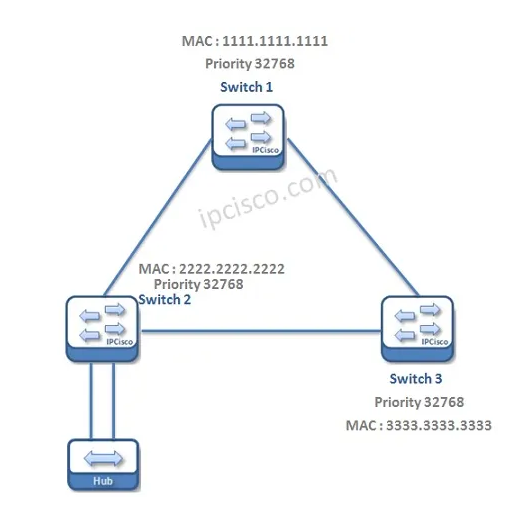
\includegraphics[width=0.7\linewidth]{screenshot002}
	\caption{}
	\label{fig:screenshot002}
\end{figure}

Aquí, se designará el puerto del puente raíz y el puerto de menor costo para el puente raíz en otros conmutadores será el puerto raíz.

En RSTP, se determinan dos puertos de bloqueo diferentes como mencionamos anteriormente. Aquí, el puerto de bloqueo en otro conmutador que no sea el puerto designado se seleccionará como puerto alternativo. Y el puerto de bloqueo en el mismo switch o segmento, será seleccionado como Puerto de Respaldo.
\begin{figure}[ph!]
	\centering
	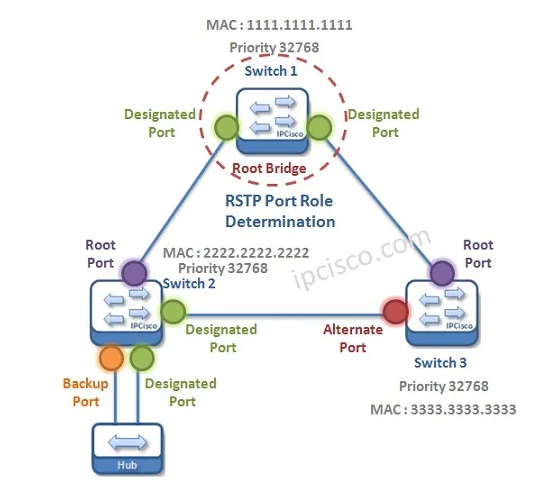
\includegraphics[width=0.7\linewidth]{screenshot003}
	\caption{}
	\label{fig:screenshot003}
\end{figure}


Interoperabilidad RSTP y STP
\\
Por último, mencionemos la interparabilidad de RSTP y STP. En diferentes redes, estos protocolos pueden funcionar juntos.

RSTP y STP son dos protocolos similares. En su red, puede haber conmutadores que admitan ambos protocolos de capa 2. Pero, ¿qué pasa si un conmutador de la red no admite RSTP? La respuesta es fácil. La topología LAyer 2 funciona únicamente con STP.

\section{¿Qué significan las letras DORA que aparecen al ejecutar ip dhcp
en los clientes?. Detalle el procedimiento indicado por esas iniciales.}

Las letras "DORA" se refieren a un acrónimo utilizado en el contexto de la asignación de direcciones IP a través del protocolo DHCP (Dynamic Host Configuration Protocol). Cada letra en "DORA" representa una etapa en el proceso de asignación de direcciones IP a un cliente DHCP. Aquí está el significado de cada letra:

D - Discover (Descubrimiento):
En esta etapa, cuando un dispositivo cliente se conecta a una red y necesita obtener una dirección IP, envía un paquete llamado "DHCP Discover". Este paquete se difunde en la red local o se envía a través de un agente relay DHCP si está configurado. El objetivo es descubrir un servidor DHCP disponible en la red.

O - Offer (Oferta):
Después de recibir el DHCP Discover, uno o más servidores DHCP en la red responden con un paquete llamado "DHCP Offer". Este paquete contiene una dirección IP que el servidor está dispuesto a asignar al cliente, junto con otros parámetros de configuración, como la máscara de subred y la dirección del servidor DNS. El cliente puede recibir múltiples ofertas de diferentes servidores DHCP si están disponibles.

R - Request (Solicitud):
Una vez que el cliente recibe las ofertas de los servidores DHCP, elige una de ellas y envía un paquete llamado "DHCP Request" al servidor seleccionado. En este paquete, el cliente solicita la dirección IP específica que se le ofreció en la etapa anterior.

A - Acknowledge (Reconocimiento):
Finalmente, el servidor DHCP que recibió la solicitud del cliente responde con un paquete "DHCP Ack" o "DHCP NAK" (si la solicitud no puede ser satisfecha). Si el servidor acepta la solicitud, envía un "DHCP Ack" al cliente, confirmando la asignación de la dirección IP y proporcionando los detalles de la configuración. En este punto, el cliente ha completado el proceso de asignación de IP y puede utilizar la dirección IP asignada.

Estas cuatro etapas, representadas por las letras "DORA," describen el proceso básico que sigue un cliente DHCP para obtener una dirección IP y otros parámetros de configuración de la red. Este protocolo es esencial para simplificar la administración de direcciones IP en redes, ya que permite la asignación dinámica y automática de direcciones IP a dispositivos en una red sin requerir configuración manual en cada dispositivo.

\section{¿Por que el cliente utiliza la dirección IP 0.0.0.0? ¿Por qué envía
	sus mensajes a la direcci´on de broadcast}

	El cliente DHCP utiliza la dirección IP 0.0.0.0 en el campo de dirección IP de origen de sus mensajes DHCP por dos razones principales:
	
	Dirección IP de origen desconocida o no asignada: Cuando un dispositivo cliente se inicia por primera vez en una red o no tiene una dirección IP asignada, utiliza la dirección IP 0.0.0.0 como dirección de origen en su mensaje DHCP Discover. Esto indica al servidor DHCP que el cliente aún no tiene una dirección IP válida y necesita que se le asigne una.
	
	Solicitud de asignación de dirección IP: El cliente envía su mensaje DHCP Discover a la dirección de broadcast (255.255.255.255) o a la dirección de broadcast limitada de su subred, dependiendo de cómo esté configurada la red. Esto se hace para asegurarse de que todos los servidores DHCP en la red reciban el mensaje. La dirección de broadcast se utiliza en lugar de una dirección IP específica porque el cliente aún no tiene una dirección IP válida y no sabe a qué servidor DHCP debe dirigirse. Enviando el mensaje a la dirección de broadcast, garantiza que todos los servidores DHCP disponibles en la red tengan la oportunidad de responder con una oferta de dirección IP.
	
	En resumen, el uso de la dirección IP 0.0.0.0 y la dirección de broadcast en los mensajes DHCP Discover es una parte fundamental del proceso de descubrimiento y asignación de direcciones IP dinámicas, ya que permite que los clientes DHCP sin direcciones IP previamente asignadas inicien el proceso y reciban ofertas de servidores DHCP en la red.
	\section{¿Se pueden conectar las PCs entre las diferentes VLANs? ¿Por qué?}

	No, porque no hay ruteo.
	\section{Que otra información provee un servidor DHCP}
	El servidor DHCP es capaz de proporcionar una variedad de información adicional a sus clientes además de la dirección IP y la puerta de enlace predeterminada (default gateway). Algunos de los datos más comunes que puede proporcionar un servidor DHCP incluyen:
	
	Máscara de subred (Subnet Mask): La máscara de subred determina qué parte de la dirección IP corresponde a la red y qué parte corresponde al host. Es esencial para que los dispositivos en la red sepan cómo enrutar el tráfico correctamente.
	
	Servidores DNS (Domain Name System): El servidor DHCP puede proporcionar las direcciones IP de uno o varios servidores DNS a los clientes. Esto permite que los dispositivos resuelvan nombres de dominio en direcciones IP, lo que es fundamental para la navegación web y otras funciones de red.
	
	Servidores WINS (Windows Internet Name Service): En entornos de red heredados de Windows, el servidor DHCP puede proporcionar las direcciones IP de los servidores WINS. WINS se utiliza para resolver nombres NetBIOS a direcciones IP.
	
	Servidores NTP (Network Time Protocol): El DHCP puede proporcionar la dirección IP de un servidor de tiempo, lo que permite a los dispositivos en la red sincronizar sus relojes para garantizar la consistencia de la hora en toda la red.
	
	Configuración de proxy (Proxy Configuration): En algunos casos, se puede configurar un servidor DHCP para proporcionar la configuración de proxy para permitir el acceso a Internet a través de un servidor proxy.
	
	Opciones personalizadas (Custom Options): Los servidores DHCP también pueden ser configurados para proporcionar información personalizada o configuraciones específicas de la red, como rutas estáticas, servidores de impresión, configuraciones de calidad de servicio (QoS), etc.
	
	Duración de la concesión (Lease Duration): El servidor DHCP especifica cuánto tiempo un cliente puede utilizar la dirección IP asignada antes de tener que renovar la concesión. Esto se conoce como el tiempo de concesión.
	
	Información del servidor (Server Identifier): El servidor DHCP puede proporcionar su propia dirección IP como identificador de servidor para que el cliente sepa a qué servidor enviar solicitudes de renovación o liberación.
	
	Nombre del dominio (Domain Name): Puede proporcionar el nombre del dominio que los clientes deben utilizar en la resolución de nombres.
	
	Rutas predeterminadas (Static Routes): En algunos casos, se pueden configurar rutas estáticas en el servidor DHCP para dirigir el tráfico hacia redes específicas.
	
	La información exacta proporcionada por el servidor DHCP puede variar según la configuración específica de la red y las necesidades del administrador. Estos son ejemplos comunes de información que un servidor DHCP puede entregar a sus clientes para facilitar la configuración y el funcionamiento de la red.
	\section{¿Qué otros mensajes se encuentran en DHCP y para qué sirven?}
	El protocolo DHCP (Dynamic Host Configuration Protocol) utiliza varios mensajes para realizar la asignación dinámica de direcciones IP y la configuración de red en una red. Los mensajes más importantes en DHCP son los siguientes:
	
	DHCP Discover (Descubrimiento DHCP): El cliente DHCP envía este mensaje para descubrir servidores DHCP disponibles en la red. Es el primer paso en el proceso de adquisición de una dirección IP.
	
	DHCP Offer (Oferta DHCP): Los servidores DHCP responden al DHCP Discover con un mensaje DHCP Offer. En esta oferta, un servidor DHCP propone una dirección IP y otros parámetros de configuración al cliente.
	
	DHCP Request (Solicitud DHCP): El cliente DHCP selecciona una de las ofertas recibidas y envía un mensaje DHCP Request al servidor DHCP elegido. Este mensaje confirma la elección del cliente y solicita formalmente la asignación de la dirección IP y la configuración.
	
	DHCP Ack (Confirmación DHCP): El servidor DHCP seleccionado responde con un mensaje DHCP Ack para confirmar la asignación de la dirección IP y la configuración al cliente. Este mensaje también incluye la duración de la concesión (lease) y otros detalles de configuración.
	
	DHCP Nak (Negación DHCP): Si el servidor DHCP no puede asignar la dirección IP solicitada por el cliente, envía un mensaje DHCP Nak para indicar al cliente que la dirección IP no está disponible. El cliente debe reiniciar el proceso de asignación.
	
	DHCP Decline (Rechazo DHCP): El cliente envía este mensaje si detecta que la dirección IP que le ha sido asignada previamente ya está en uso en la red. El servidor DHCP puede liberar la dirección IP y volver a ponerla en disponibilidad.
	
	DHCP Release (Liberación DHCP): Cuando un cliente ya no necesita una dirección IP o se desconecta de la red, envía un mensaje DHCP Release para liberar la dirección IP y notificar al servidor DHCP que está disponible para ser asignada a otros clientes.
	
	DHCP Inform (Información DHCP): Los clientes pueden enviar un mensaje DHCP Inform para obtener información adicional de configuración sin solicitar una dirección IP nueva. Esto puede incluir información sobre opciones de configuración o actualizaciones de parámetros existentes.
	
	DHCP Option 82: Aunque no es un mensaje DHCP en sí mismo, la opción 82 se utiliza para proporcionar información adicional sobre la ubicación física del cliente en la red. Es útil en entornos de red más complejos y permite una asignación más granular de direcciones IP.
	
	En resumen, estos mensajes DHCP permiten que los clientes y servidores DHCP negocien y gestionen la asignación de direcciones IP y la configuración de red de manera dinámica. Cada mensaje cumple un propósito específico en el proceso de configuración de red y asegura que los dispositivos obtengan las direcciones y configuraciones adecuadas para su funcionamiento en la red.